\documentclass[10pt,a4paper,catalan]{article}
\usepackage[latin1]{inputenc}
%\usepackage[T1]{fontenc}
\usepackage{babel}
\usepackage[a4paper,left=2cm,right=2cm,top=3cm,bottom=3cm]{geometry}
%\usepackage{amsmath}
%\usepackage{amsfonts}
%\usepackage{amssymb}
\usepackage[pdftex,bookmarks=true,pdfborder={000}]{hyperref}
\usepackage{xcolor}
\usepackage{listings}
%\usepackage{caption}
\usepackage{graphicx}
\usepackage{float}
\usepackage{subfig}


\DeclareCaptionFont{white}{\color{white}}
\DeclareCaptionFormat{listing}{\colorbox{gray}{\parbox{\textwidth}{#1#2#3}}}
\captionsetup[lstlisting]{format=listing,labelfont=white,textfont=white}

\definecolor{gray97}{gray}{.97}
\definecolor{gray75}{gray}{.75}
\definecolor{gray45}{gray}{.45}

\lstset{
  frame=Ltb,
  language=C,
  captionpos=t,
  tabsize=2,
  framerule=0pt,
  framextopmargin=5pt,
  framexbottommargin=3pt,
  framexleftmargin=0.4cm,
  framesep=0pt,
  rulesep=.4pt,
  backgroundcolor=\color{gray97},
  rulesepcolor=\color{black},
  showstringspaces = false,
  keywordstyle=\bfseries\color{blue},
  commentstyle=\color{teal},
  stringstyle=\ttfamily\color{red},
  numbers=left,
  numbersep=15pt,
  numberstyle=\tiny,
  numberfirstline = false,
  breaklines=true,
  showstringspaces=false,
  basicstyle=\ttfamily\footnotesize,
  emph={label}
}

\newcommand{\unit}[1]{\ensuremath{\, \mathrm{#1}}}

%opening
\title{Pr\'actica 3: Control de instrumentos a bajo nivel. Peticiones de servicio}
\author{Dani Gabriel y Rafael G\'omez}
\date{Marzo 2011}

\begin{document}

\pagebreak

\maketitle

\tableofcontents

\pagebreak

\section{Estudio previo}

\begin{figure}[H]
 \centering
 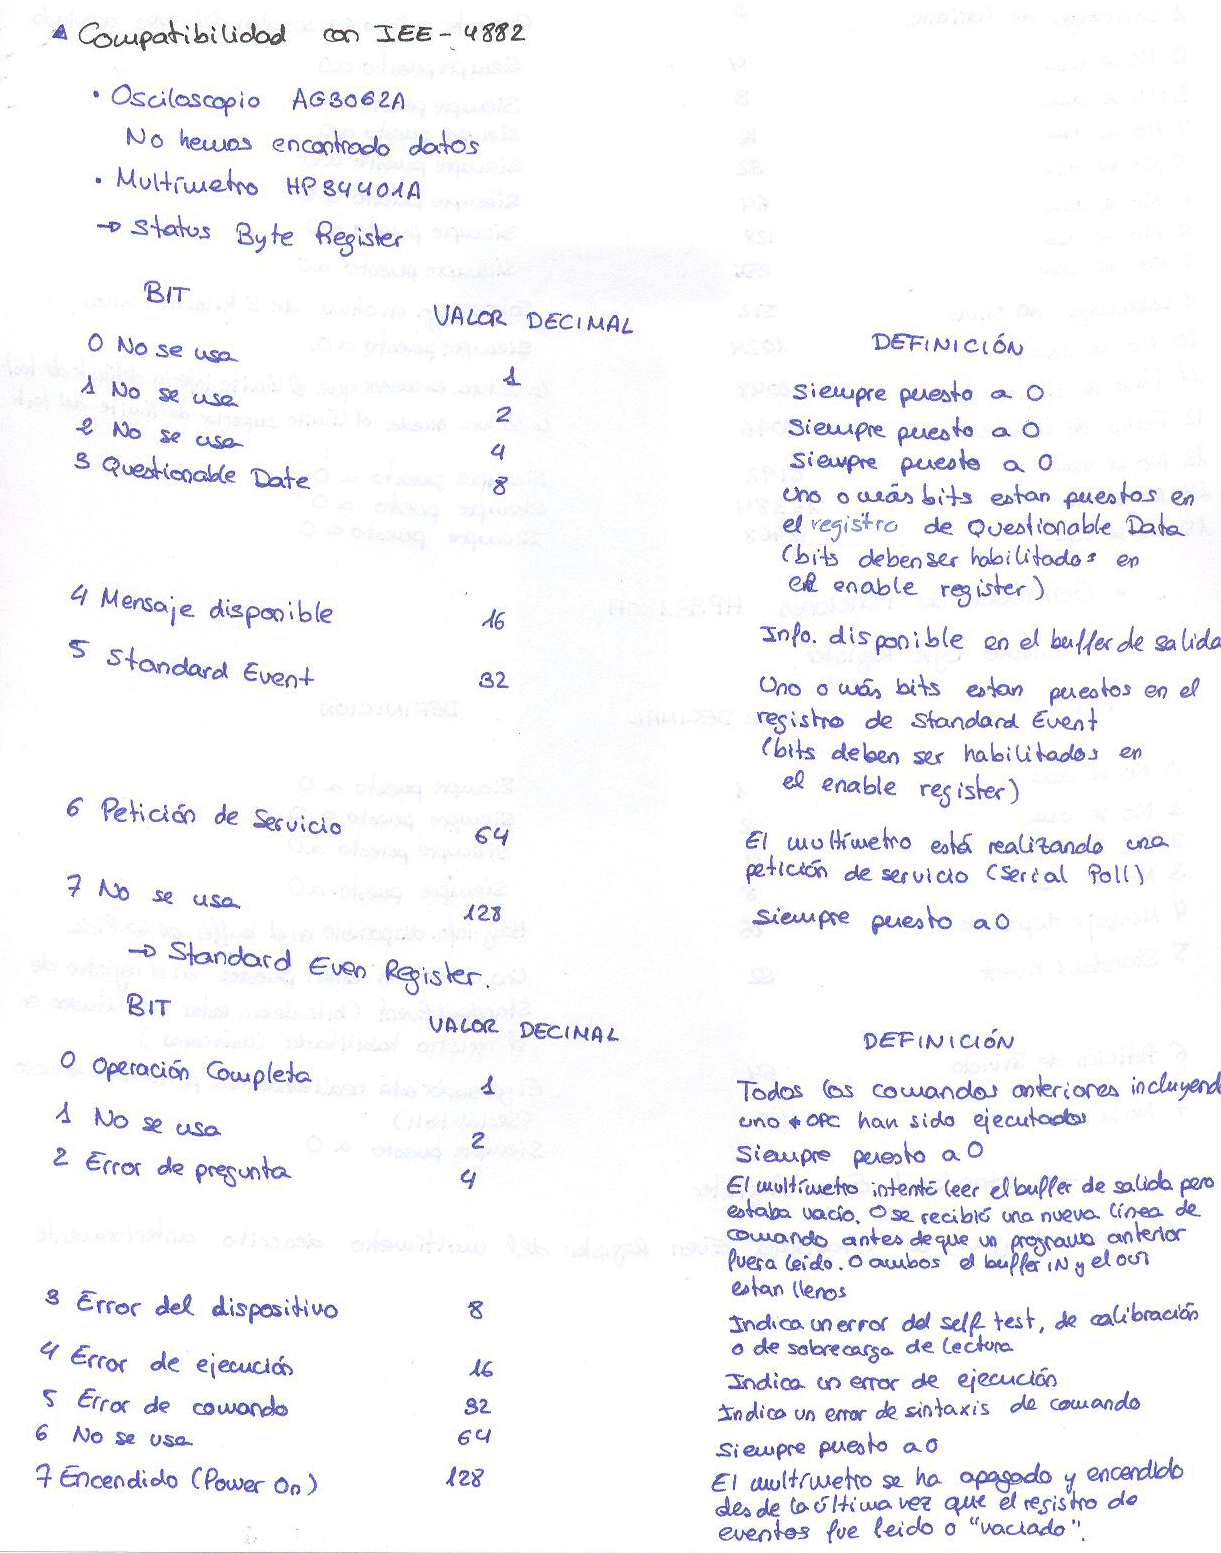
\includegraphics[width=1\textwidth]{previos1}
\end{figure} 

\begin{figure}[H]
 \centering
 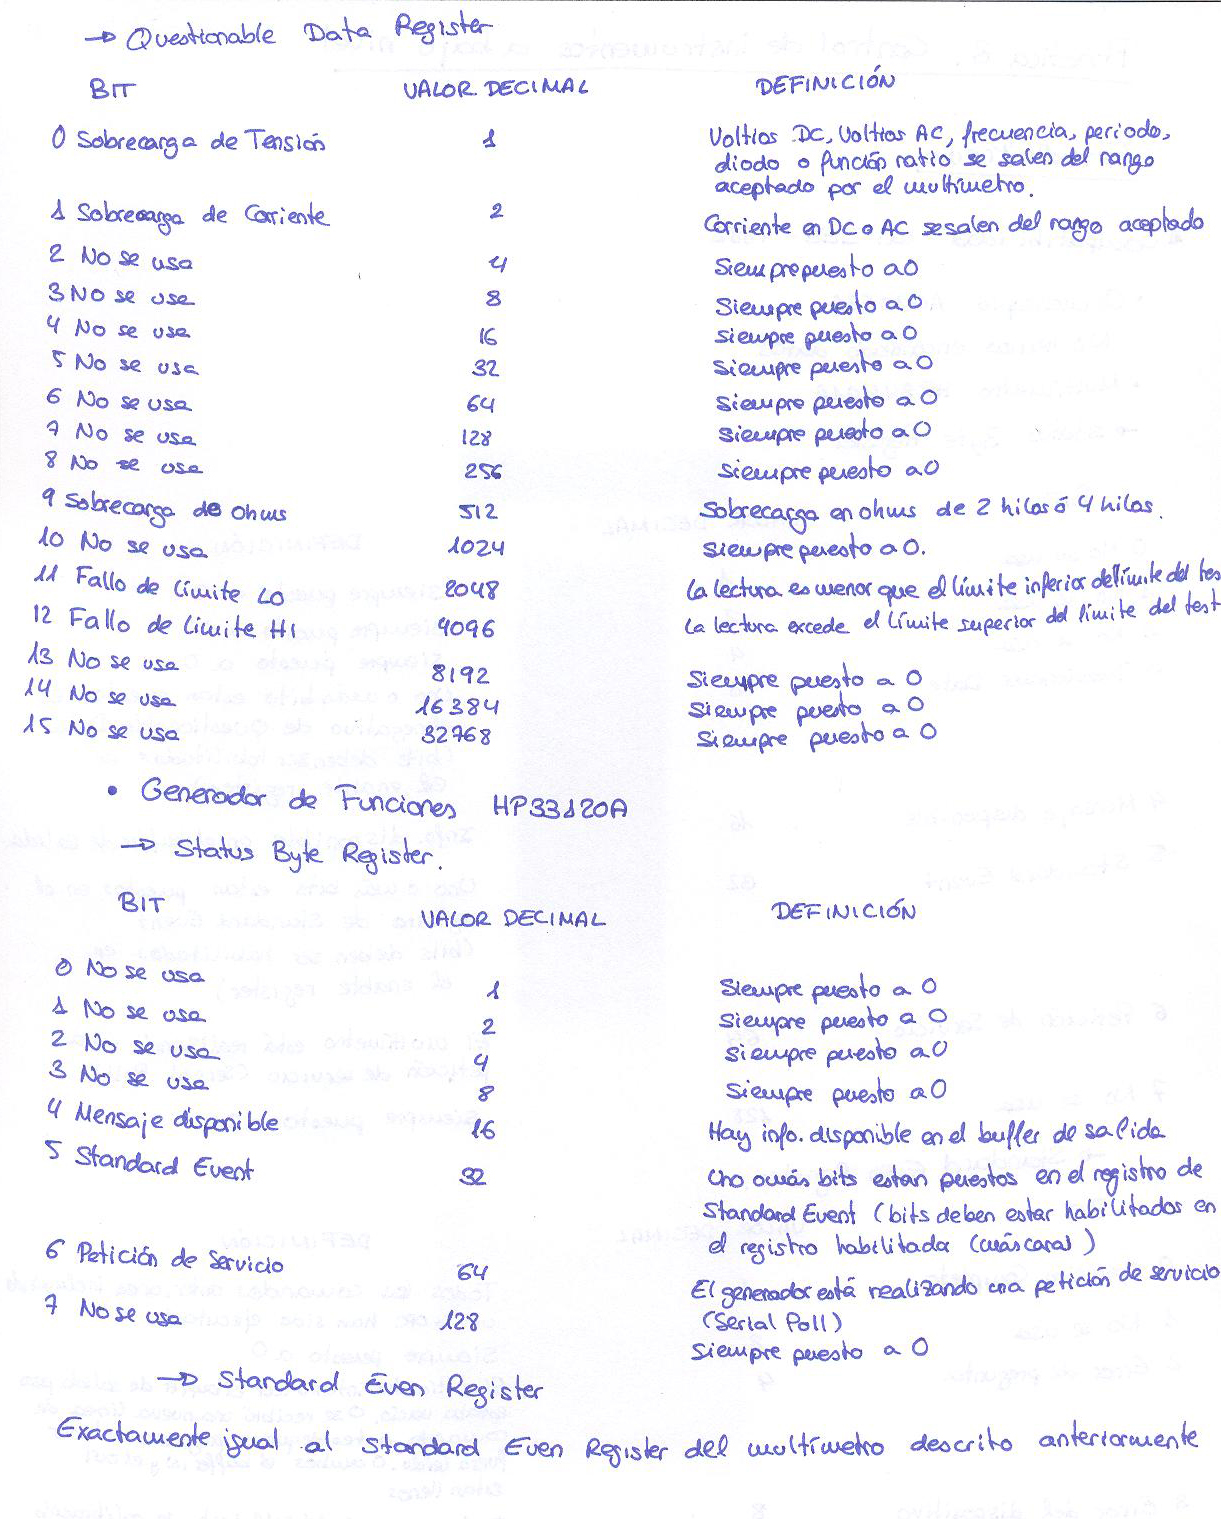
\includegraphics[width=1\textwidth]{previos2}
\end{figure}
  
\begin{figure}[H]
 \centering
 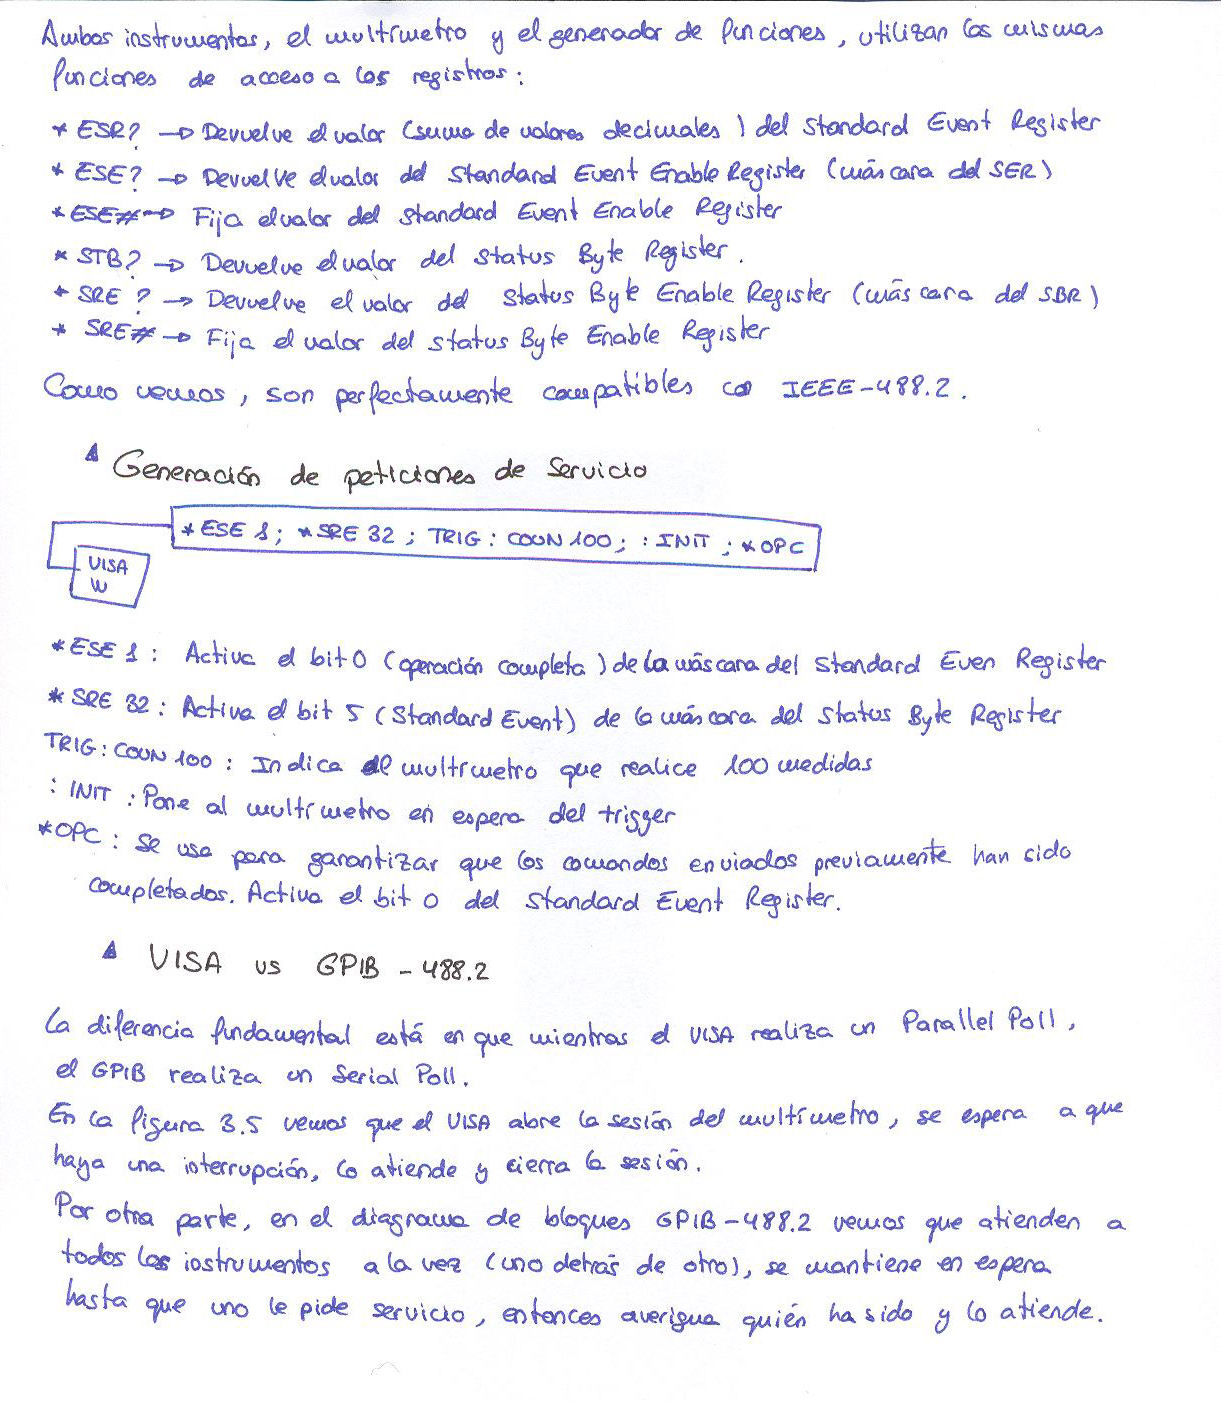
\includegraphics[width=1\textwidth]{previos3}
\end{figure}

\section{Trabajo de Laboratorio}

\subsection{Realizaci�n autom�tica de medidas con el mult�metro}

En este apartado se pretende programar el mult�metro para que realice una serie de 100 medidas de tension (AC) y calcule la media, el valor m�ximo y el m�nimo y lo presente por pantalla.

Rellenamos los campos del \emph{draft} que se nos proporciona y comprovamos el correcto funcionamiento del programa.Ver figura \ref{fig:aver}.

\begin{figure}[H]
 \centering
 \subfloat[Diagrama de bloques]{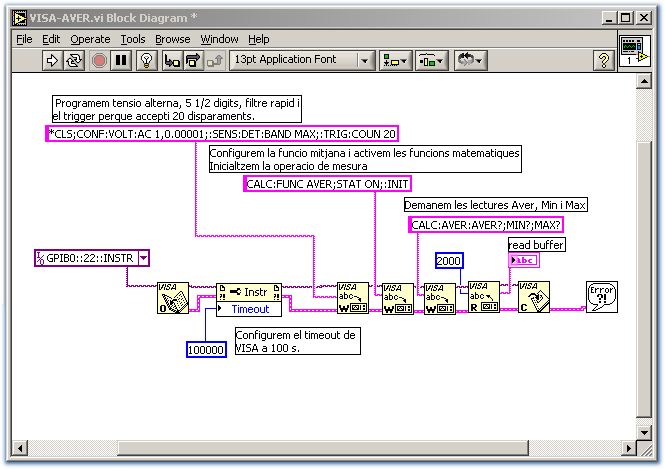
\includegraphics[width=0.6\textwidth]{bloqAver}}
 \vspace{0.5cm}
 \subfloat[Panel frontal]{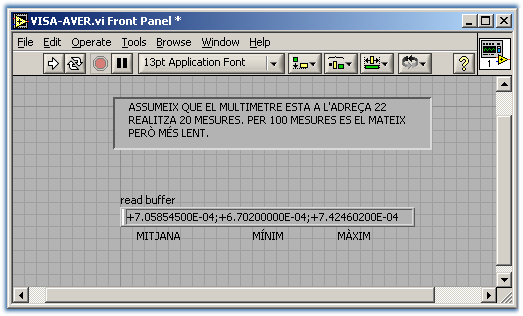
\includegraphics[width=0.6\textwidth]{frontAver}}
 \vspace{0.3cm}
 \caption{Realizaci�n de las medidas}
 \label{fig:aver}
\end{figure}

\subsection{Detecci�n de la finalizaci�n de las medidas}

En este apartado realizaremos las mismas medidas que en el anterior, pero detectaremos cu�ndo el instrumento ha finalizado la operaci�n y tiene un nuevo dato en el registro de salida mediante interrupciones. En el manual de pr�cticas hay una explicaci�n detallada del protocolo que hay que seguir en los registros y flags propios del mult�metro.

Despu�s de rellenar el \emph{draft} del diagrama de bloques que se nos proporciona, el resultado es el que queda en la figura \ref{fig:srq}

\begin{figure}[H]
 \centering
 \subfloat[Diagrama de bloques]{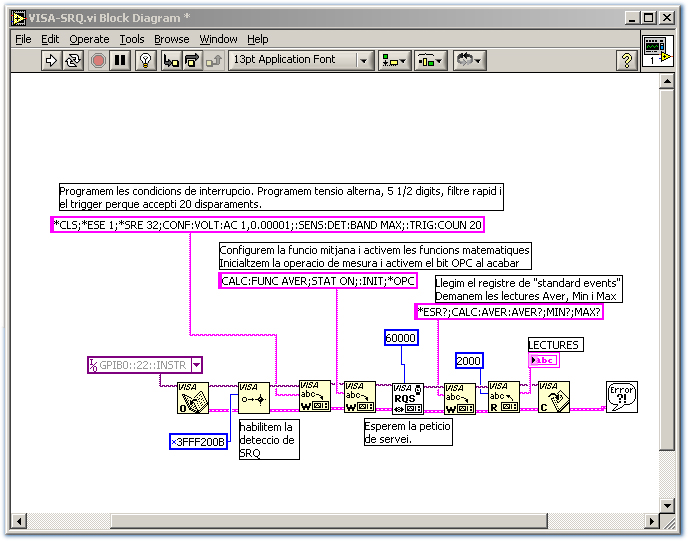
\includegraphics[width=0.6\textwidth]{bloqSRQ}}
 \vspace{0.5cm}
 \subfloat[Panel frontal]{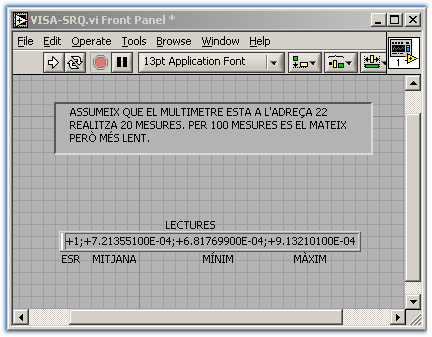
\includegraphics[width=0.6\textwidth]{frontSRQ}}
 \vspace{0.3cm}
 \caption{Realizaci�n de las medidas mediante interrupciones}
 \label{fig:srq}
\end{figure}


\end{document}